\documentclass[11pt]{article}
\usepackage[margin=1in]{geometry}
\usepackage{booktabs,multirow,amsmath,amssymb,graphicx,xcolor,url}
\usepackage[numbers,sort&compress]{natbib}
\usepackage{hyperref}

\title{REVA: Region-Evidence Arbitration with Vocabulary-Adaptive\\
Background Synthesis for Plain-Vocabulary Robustness\\
in Training-free Open-Vocabulary Segmentation}
\author{Thomas Sam\thanks{Author list and affiliations to be finalized before submission.}}
\date{July 31, 2026}

\newcommand{\miou}{mIoU}
\newcommand{\reva}{REVA}

\begin{document}
\maketitle

\begin{abstract}
Training-free open-vocabulary semantic segmentation (OVSS) methods lose 12--21 \miou{}
when the carefully engineered benchmark vocabulary is replaced by the plain class names
a real user would type. We present \reva{}, a training-free, plug-in inference procedure
that recovers this gap for \emph{arbitrary} plain vocabularies. We scope the
robustness claim to the plain-naming axis; the audit's other axes (synonyms,
adversarial naming) are measured rather than claimed. \reva{} combines two
components: (i) \emph{vocabulary-adaptive background synthesis} (VABS), which selects a
covering set of scene/stuff negative queries for the user's vocabulary via
facility-location optimization with a similarity safety filter, and (ii)
\emph{region-evidence arbitration}, which averages dense per-pixel class probabilities
inside SAM automasks and re-assigns each region by pooled evidence, with pixel-level
fallback. On PASCAL VOC-21 (validation split excluding our development images),
\reva{} lifts four training-free methods (MaskCLIP, SCLIP, ClearCLIP, NACLIP) from
plain-vocabulary baselines by $+19.9$ to $+23.1$ \miou{}, closing 86--96\% of the gap to
a matched-compute engineered-vocabulary upper bound (official vocabulary with the same
region arbitration), and adds $+4$ to $+9$ \miou{} on top of the official
vocabulary itself. Every design decision was pre-registered with kill criteria and matched
controls: the selection advantage over matched random negatives is
positive in all 6 seeded cells on the full evaluation split (3 seeds, mean
$+3.1$/$+3.6$ under region arbitration on SCLIP/NACLIP, range $+1.2$ to
$+5.1$), and region arbitration
passes the pre-registered no-added-harm criterion over pixel-level VABS
(no class drops more than 3 IoU on two or more methods; worst single-method
regression $-3.2$). External validity is anchored on unmodified official
releases: VABS transfers to four official codebases (ProxyCLIP, SC-CLIP,
Trident, CorrCLIP), and on SC-CLIP the full pipeline recovers 93\% of the
author-code naming-engineering gap. We report the boundaries equally: a
pre-registered self-attack shows a tuned scalar background boost reproduces
73--85\% of VABS's text-side gain (VABS's residual, untuned advantage is
$+2.8$ to $+4.4$); the engineered vocabulary retains a 0.9--3.6 \miou{}
advantage under matched compute; SAM dominates runtime
($\sim$12$\times$ the CLIP pass); on Context-60 the negative-selection
advantage vanishes; and a hand-written VOC background expansion matches VABS
on VOC while losing to it off-VOC. The contribution is thus automation and
vocabulary robustness, not a claim of a superior mechanism: \reva{} approaches
hand-engineered-vocabulary quality with zero manual vocabulary work.
\end{abstract}

\section{Introduction}

Training-free OVSS methods \citep{zhou2022maskclip,wang2024sclip,lan2024clearclip,
hajimiri2024naclip} adapt CLIP \citep{radford2021clip} to dense prediction and are
evaluated with fixed benchmark vocabularies. A controlled audit
\citep{sam2026fragile} showed that these official vocabularies embed undocumented
engineering---background query expansion and positive sub-class expansion---worth
11.8--20.6 \miou{} on VOC-21, and that no pre-registered \emph{text-only} mechanism
could recover the engineered value safely: synthesised background negatives recovered
the macro gap but systematically harmed classes such as \emph{person} and
\emph{tvmonitor}, because harmful negatives are textually distant yet visually close,
which no text-similarity filter can detect.

This paper provides the constructive answer that the audit predicted would require
\emph{independent visual evidence}. We arbitrate the competition between target
classes and synthesised negatives at the level of visual regions rather than pixels:
class-probability evidence is averaged inside SAM \citep{kirillov2023sam} automasks,
and each region is assigned by pooled evidence. An oracle diagnostic motivates the
design: pooling over ground-truth regions separates previously harmed target regions
from background regions with AUC $0.92$--$0.97$ under the same vocabulary in which
pixel-level evidence failed, and the failure of a superpixel variant (SLIC) shows that
region \emph{quality}, not pooling itself, is the operative ingredient.

Our contributions:
\begin{enumerate}
\item \textbf{\reva{}}, a training-free plug-in that makes arbitrary plain
vocabularies usable: vocabulary-adaptive background synthesis (facility-location
selection over a scene/stuff lexicon with a similarity safety filter) plus SAM-region
probability pooling with pixel fallback. No fine-tuning, no SAM decoder re-prompting,
no mask-discovery heuristics.
\item \textbf{A pre-registered evidence chain} with matched controls: every stage was
frozen before test runs, with kill criteria; two of our own stages (SLIC pooling and a
DINOv2 visual veto) were killed by their criteria and are reported as negative
results.
\item \textbf{Honest boundary mapping}: matched random negatives isolate the
selection advantage; under matched compute the engineered vocabulary keeps a
0.9--3.6 \miou{} lead (\reva{} closes 86--96\% of the gap, it does not eliminate it); a
hand-written-background control shows \reva{} \emph{matches} manual engineering
on VOC-21 rather than exceeding it (while beating the same list transplanted
off-VOC); a LaVG-style feature-pooling variant performs on par with
probability pooling; against the plain baseline, person and tvmonitor remain harmed
(bounded, disclosed per class); and on Context-60 the selection advantage disappears.
\end{enumerate}

\section{Related Work}

\paragraph{Training-free OVSS.} Trained open-vocabulary segmenters align masks to
language with segmentation or image-text supervision
\citep{li2022lseg,xu2022groupvit,liang2023ovseg,xu2023san,cho2024catseg}; the
training-free line instead re-reads a frozen CLIP \citep{radford2021clip}.
MaskCLIP \citep{zhou2022maskclip} re-projects CLIP's
value features; SCLIP \citep{wang2024sclip} and ClearCLIP \citep{lan2024clearclip}
modify final-block attention; NACLIP \citep{hajimiri2024naclip} adds neighbourhood
priors. \reva{} is a plug-in on top of any of them.

\paragraph{SAM/visual evidence in OVSS.} Prior work couples SAM with CLIP either by
training fusion modules (SAM-CLIP \citep{wang2024samclip}, OVSAM \citep{yuan2024ovsam},
ESC-Net \citep{lee2025escnet}), by prompt-based re-decoding of coarse predictions
(Trident \citep{shi2025trident}), or by ensembling automasks with CRF outputs (CaR
\citep{sun2024car}); LaVG \citep{kang2024lavg} grounds text on unsupervised Ncut masks
via feature-prototype similarity, and ProxyCLIP \citep{lan2024proxyclip} injects
SAM/DINO features as attention proxies. \reva{} instead performs output-level
arbitration by averaging dense per-pixel class \emph{probabilities} inside SAM
automasks with pixel-level fallback, leaving encoders and the base method untouched.
We do not claim novelty for region pooling itself---our ablation shows LaVG-style
feature pooling performs comparably on SAM masks---but for the combination with
vocabulary-adaptive negatives and its effect on vocabulary robustness.

\paragraph{Background modelling.} Hand-written background query lists are folklore
(SCLIP, CaR, LaVG); OVDiff \citep{karazija2024ovdiff} synthesises visual negative
prototypes with a diffusion model; TCC \citep{tcc2024} derives test-time contrastive
concepts for single-concept segmentation. VABS synthesises a negative set for
arbitrary \emph{multi-class} plain vocabularies by facility-location coverage
optimization over a fixed scene/stuff lexicon with a similarity safety filter. A same-protocol
anchor against Trident's SAM-refinement stage and PAMR is reported in
Table~\ref{tab:anchor}; a TCC comparison remains future work
(\S\ref{sec:limitations}).

\paragraph{Vocabulary robustness.} On the classification side, prompt and name
phrasing are long known to shift zero-shot accuracy
\citep{radford2021clip,zhou2022coop,pratt2023cupl,roth2023waffle}. For
segmentation, the audit \citep{sam2026fragile} established the
protocol and the plain-vs-official gap that \reva{} closes. Image-conditional
vocabulary \emph{pruning} (FreeCP \citep{freecp2025}; concurrently ActiveSAM
\citep{activesam2026} on the SAM~3 concept-prompt stack) subtracts classes to
reduce false-positive competition, whereas VABS \emph{adds} negatives to
repair background under-modelling --- orthogonal interventions on the
inference vocabulary (our own detector-guided pruning candidate,
\S\ref{sec:prune}, is of the former kind). Concurrent SynCLIP
\citep{wang2026synclip} obtains synonym robustness by synonym-coherent
re-pretraining of the encoders; \reva{} is a pure inference-time plug-in and
targets a gap (plain-vs-engineered background modelling) that re-pretraining
does not address. Concurrent PTC \citep{ptc2026} calibrates the \emph{text}
embeddings of the given classes with visual prototypes, modulating calibration
strength per image and class by evidence amount; it introduces no background
negatives and no label-free applicability signal (its dataset-level dial is
tuned with labels, nearly closing on COCO-Object with $\mu{=}0.02$ vs
$0.15$--$0.35$ elsewhere), and it reports no
switch-off rule for the harmful regime it observes there --- independently
corroborating the low-headroom boundary we characterise, while intervening on
an orthogonal quantity.

\section{Method}
\label{sec:method}

\begin{figure}[t]
\centering
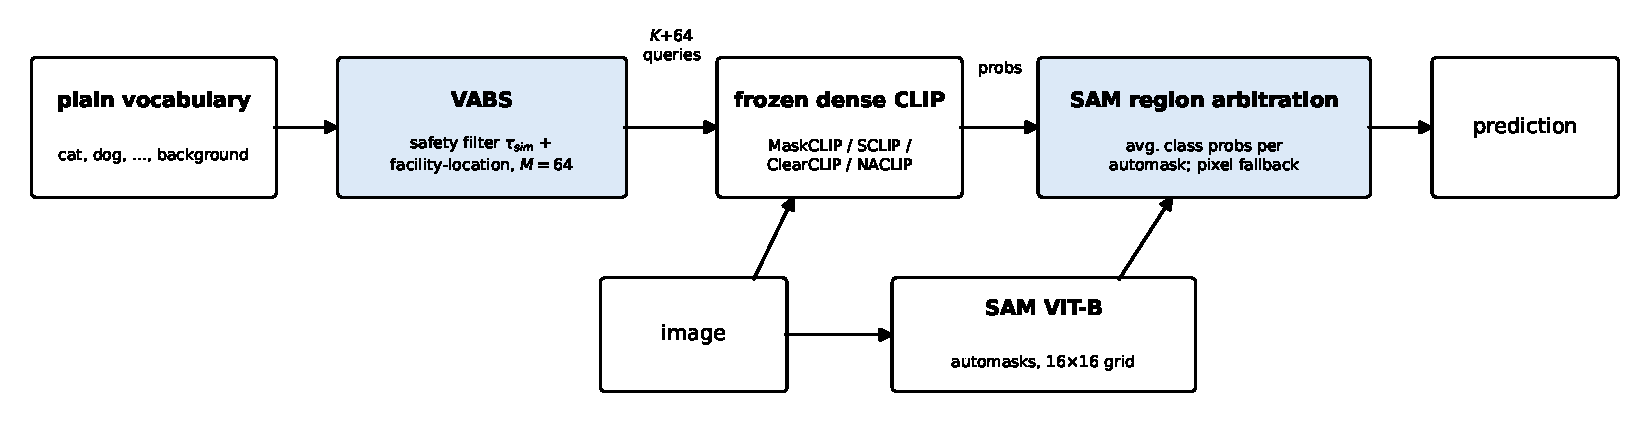
\includegraphics[width=\linewidth]{figs/reva_pipeline.pdf}
\caption{\reva{} overview. Both components are training-free and leave the base
method untouched: VABS synthesises vocabulary-conditioned background negatives
(blue); SAM automasks arbitrate target/negative competition by pooled probability
evidence (blue). Pixels covered by no mask keep their pixel-level prediction.}
\label{fig:overview}
\end{figure}

\paragraph{Setting.} A frozen training-free OVSS method produces dense patch
embeddings aligned to CLIP text space. The user supplies $K$ plain class names
(including a bare ``background''). Text queries use the standard 80-template mean
embedding \citep{radford2021clip}; multi-word entries joined by commas act as sub-queries of one class with
max-pooled probabilities (SCLIP convention).

\paragraph{VABS: vocabulary-adaptive background synthesis.} Given target embeddings
$T\in\mathbb{R}^{K\times d}$ and a scene/stuff lexicon $L$ (COCO-Stuff
\citep{caesar2018cocostuff} $\cup$ ADE-150 \citep{zhou2017ade} class names, 168 entries after splitting and de-duplication), VABS (i) removes
candidates with $\max_k \cos(t_c, T_k) \ge \tau_{\mathrm{sim}}=0.90$ (safety filter),
then (ii) greedily selects $M=64$ negatives by facility-location coverage
\citep{krause2014submodular} of the remaining candidate space with a redundancy penalty. Selected negatives become
sub-queries of the background class: any pixel they win is background. Hyper-parameters
$(M,\tau_{\mathrm{sim}})$ were fixed on a 100-image development split (disjoint from
all test images) in earlier pre-registered work and never re-tuned.

\paragraph{Why discrete negatives and per-patch max.} Two pre-registered
probes fix the aggregation choice mechanistically. Replacing the discrete
negative set by a continuous background \emph{subspace} (projection-norm
energy of the patch feature onto the top-$32$ singular directions of the
lexicon embeddings, scale-anchored per image) collapses to the plain
baseline ($34.5$/$34.4$ vs $53.6$/$52.7$ for the discrete set on
SCLIP/NACLIP, VOC test-300): a global energy scalar is nearly uniform
across patches and carries no per-patch discrimination. A follow-up sweep
interpolating between the two --- background score $=$ mean of the top-$k$
negative probabilities, $k\in\{1,2,4,8,16,64\}$ --- degrades
\emph{monotonically} with $k$ on all three hosts and both datasets (e.g.\
SCLIP VOC $53.6 \to 52.7 \to 50.7 \to 47.0 \to 40.5 \to 27.2$; $k{=}64$,
the discrete analogue of the energy score, falls below plain), and the
winning negative is patch-dependent beyond a handful of words: on $50$
VOC images per host, the eight globally most frequent winners cover only
$58$--$64\%$ of background-won patches; and a follow-up pre-registered
pruning test shows the coverage is not the whole story --- keeping only
the global top-$24$ winners (which cover ${\sim}92\%$ of wins on the
VOC diagnostic images) still loses against the
full set by $0.58$--$1.12$ \miou{} in five of six host--dataset cells
(the sixth loses $0.46$, just inside the frozen $0.5$ bar), so
lower-ranked negatives contribute
through runner-up competition beyond their win counts. The background channel therefore needs per-patch
discrete competition against the full diverse set; every averaging- or
pruning-based alternative we froze in advance performs worse (single
seed, shared CLIP backbone across hosts; run records in the artifact).

\paragraph{Region-evidence arbitration.} SAM (ViT-B, automatic mask generation,
$16\times16$ point grid) proposes class-agnostic masks on the resized image. Masks are
rasterised largest-first so smaller masks overwrite larger ones, preserving detail;
pixels covered by no mask keep their pixel-level prediction. For each region $r$ the
class-probability map (after softmax with logit scale 40 and per-class sub-query max
pooling) is averaged: $p_r = \frac{1}{|r|}\sum_{x\in r} p(x)$, and the region is
assigned $\arg\max_c p_{r,c}$.

\paragraph{Why regions, not confidence.} Our earlier text-only attempt failed because
dense CLIP confidence is diffuse: at threshold $0.5$, zero high-confidence
\emph{person} patches exist, so no pixel-level filter can protect harmed classes. The
oracle diagnostic (\S\ref{sec:oracle}) shows evidence pooled over true regions is
separable, i.e.\ information the pixel view cannot expose.

\section{Pre-registered evidence chain}
\label{sec:prereg}

All experiments run on OpenCLIP \citep{ilharco2021openclip} ViT-B/16 (OpenAI
weights), short side 336, window 224, stride 112, logit scale 40, no
post-processing (no PAMR \citep{araslanov2020}, no multi-scale/flip). Benchmarks
are PASCAL VOC-21 \citep{everingham2010voc}, PASCAL-Context-60
\citep{mottaghi2014context}, COCO-Object \citep{lin2014coco}, and ADE-150
\citep{zhou2017ade}. This
minimal unified protocol yields lower absolute numbers than published method-specific
pipelines (e.g.\ our NACLIP official-vocabulary baseline is 56.9 versus the published
64.1, which uses PAMR refinement --- resolution settings match ours); all claims in this paper are
\emph{within-protocol deltas} under identical settings across arms, not
state-of-the-art absolute comparisons. Development used 100 VOC images (validation
images 300--399); all VOC test numbers exclude these 100 images (1349 images).
Because every class occurs in the ground truth of the test images, the reported
\miou{} is the standard all-class dataset-level \miou{} computed from a globally
aggregated confusion matrix---not a per-image GT-present average, avoiding the metric
artifact documented in the audit \citep{sam2026fragile}. Criteria were frozen before
each test run; we report the chain including its kills. Throughout the paper,
gains and deltas quoted in the text are computed from unrounded run records;
they may differ from differences of the displayed values (rounded to 0.1) by
up to 0.1.

\subsection{Stage 0: oracle diagnostic and the SLIC kill}
\label{sec:oracle}
Pooling raw similarities over ground-truth connected components separates
previously-harmed target regions (person, tvmonitor) from background regions with AUC
$0.92$/$0.97$ under the VABS vocabulary---the same vocabulary under which pixel-level
evidence harmed those classes. But the same pooling over SLIC superpixels
\emph{decreased} dev \miou{} by $3.0$, killing the superpixel variant by its
pre-registered criterion and isolating region quality as the bottleneck.

\subsection{Stage 1: SAM regions (main result)}
Replacing SLIC with SAM automasks passed all frozen criteria on dev and was then
validated on the full split (Table~\ref{tab:main}).

\begin{table}[t]
\centering\small
\caption{VOC-21 validation split excluding the 100 development images (1349 images;
standard all-class \miou{} from a globally aggregated confusion matrix). ``pix'' =
pixel-level, ``+SAM'' = region-evidence arbitration. rand.\ 64 = matched random
negatives (single seed here; a 3-seed full-split replication gives a seeded
selection advantage of $+3.1$/$+3.6$ mean, positive in all cells; finding (ii) below). \reva{} = plain + VABS + SAM. Official numbers use the
engineered benchmark vocabulary; official+SAM is the matched-compute upper bound.
The audit's image-resampling noise floor on 300-image subsets is 3.1 \miou{};
this full-split table is less noisy, but sub-\miou{} differences are not interpreted.}
\label{tab:main}
\begin{tabular}{lccccccc}
\toprule
& \multicolumn{5}{c}{plain vocabulary} & \multicolumn{2}{c}{official vocabulary} \\
\cmidrule(lr){2-6}\cmidrule(lr){7-8}
Method & pix & pix+SAM & pix+VABS & rand.64+SAM & \textbf{\reva{}} & pix & +SAM \\
\midrule
SCLIP     & 35.6 & 36.6 & 55.5 & 53.6 & \textbf{58.7} & 57.2 & 61.2 \\
ClearCLIP & 34.8 & 35.2 & 52.9 & 50.2 & \textbf{56.1} & 55.7 & 59.7 \\
MaskCLIP  & 32.8 & 39.0 & 45.1 & 47.5 & \textbf{52.7} & 44.6 & 53.6 \\
NACLIP    & 36.9 & 39.6 & 54.1 & 54.5 & \textbf{59.2} & 56.9 & 62.6 \\
\bottomrule
\end{tabular}
\end{table}

Findings (dev-excluded split): (i) SAM arbitration alone barely helps the plain
vocabulary ($+0.4$ to $+6.2$; column pix+SAM)---VABS and arbitration are only strong
\emph{together}: region arbitration adds $+3.2$ to $+7.6$ over pixel-level VABS, for
a total plain$\rightarrow$\reva{} gain of $+19.9$ to $+23.1$; (ii) the selection
advantage over matched random negatives is $+4.7$ to $+5.9$ under region
arbitration (Table~\ref{tab:main}, \reva{} vs.\ rand.64$+$SAM; single seed
here); a pre-registered 3-seed replication of the
random-negative set on the \emph{full} dev-excluded split (1349 images, region
arbitration) gives seeded advantages of $+5.1$/$+1.2$/$+2.9$ (SCLIP, mean
$+3.1$) and $+4.7$/$+2.1$/$+4.0$ (NACLIP, mean $+3.6$): positive in all 6
cells. An earlier test-300 replication of the same seeds was noisier
($-0.1$ to $+3.8$, spread comparable to the 3.1 subset noise floor), so
subset-level estimates of this advantage should carry that caveat;
(iii) \reva{} on plain vocabularies exceeds the official vocabulary evaluated
\emph{at pixel level} for all four methods---but this is an unequal-compute
comparison: under matched compute (official + SAM) the engineered vocabulary retains
a 0.9--3.6 \miou{} lead, i.e.\ \reva{} closes 86--96\% of the engineered-vocabulary
gap rather than eliminating it (per method: SCLIP 90\%, ClearCLIP 86\%, MaskCLIP
96\%, NACLIP 87\%); (iv) the plug-in is orthogonal: applied on top of the official
vocabulary it still adds $+4.0$ to $+9.0$; (iv-b) a pre-registered
self-attack control (the companion audit's one-parameter test: any
absorption claim must beat a direct background calibration): even when
the competitor is handed a labelled advantage --- a \emph{single scalar
background-logit boost} tuned on a 100-image labelled dev split, where
VABS gets no per-vocabulary tuning --- VABS still wins by $2.8$--$4.4$
under the frozen criterion, and the boost adds only $+0.2$ to $+1.1$
on top of VABS. The tuned boost does reproduce 73--85\% of the
text-side VABS gain on VOC (SCLIP $34.7\to50.7$ vs VABS $53.5$; NACLIP
$36.6\to48.4$ vs $52.8$), and it is brittle (the best boost differs per
model and $+0.08$ collapses SCLIP to $33$). A pre-registered transfer
check settles whether the boost is a portable competitor: the
VOC-tuned scalar \emph{harms} on every transfer cell (Context-60
$-0.3$ to $-0.9$ on plain, $-5.8$ to $-9.6$ on top of VABS; ADE-150
$-1.3$ to $-1.4$, where the plain protocol has no background class to
boost at all) --- the boost is a dataset-specific calibration constant
requiring labelled re-tuning per benchmark, whereas untuned VABS gains
on Context-60 and only reproduces its already-disclosed ADE null.
We read VABS as automatic, vocabulary-conditioned
background re-calibration plus a genuine selection component, and
report the boost as a baseline any negative-vocabulary method should
be compared against; (v) per-class safety under the pre-registered criterion (\reva{} vs.\ pixel-level
VABS, i.e.\ does arbitration \emph{add} harm): no class drops more than 3 IoU on two
or more methods (single worst case: person $-3.2$ on NACLIP). Against the
\emph{plain} baseline, however, the harm inherited from text-only negative synthesis
is reduced but not eliminated: person remains $-6.0$/$-6.0$/$+8.6$/$-8.9$ and
tvmonitor $-2.9$/$-11.2$/$-6.3$/$-11.8$ (SCLIP/ClearCLIP/MaskCLIP/NACLIP;
Table~\ref{tab:perclass}). The same signature extends to --- and is somewhat
larger on --- the three 2024--25 style-reimplementation bases (test-300):
person $-7.7$/$-15.4$/$-13.0$ and tvmonitor $-13.9$/$-12.0$/$-13.0$ on
ProxyCLIP- \citep{lan2024proxyclip}/LPOSS- \citep{stojnic2025lposs}/SC-CLIP-style
\citep{bai2024scclip} respectively, with LPOSS tvmonitor dropping to
near zero (2.1), while pottedplant improves by $+13$ to $+18$ on all three.
\reva{} trades bounded losses on 2 of 21 classes for a
$+20$-level macro gain; users for whom person or tvmonitor is critical should not
adopt the plug-in blindly. A pre-registered attempt to \emph{predict} the
at-risk classes from text alone fails: the max text cosine of a class to the
64 selected negatives does not rank per-class deltas (Spearman $+0.37$/$+0.39$,
wrong sign vs.\ the frozen hypothesis, $p{>}0.09$; full split, 20 classes) ---
so the per-class safety table, not a text-side screen, remains the deployment
check.

\begin{figure}[t]
\centering
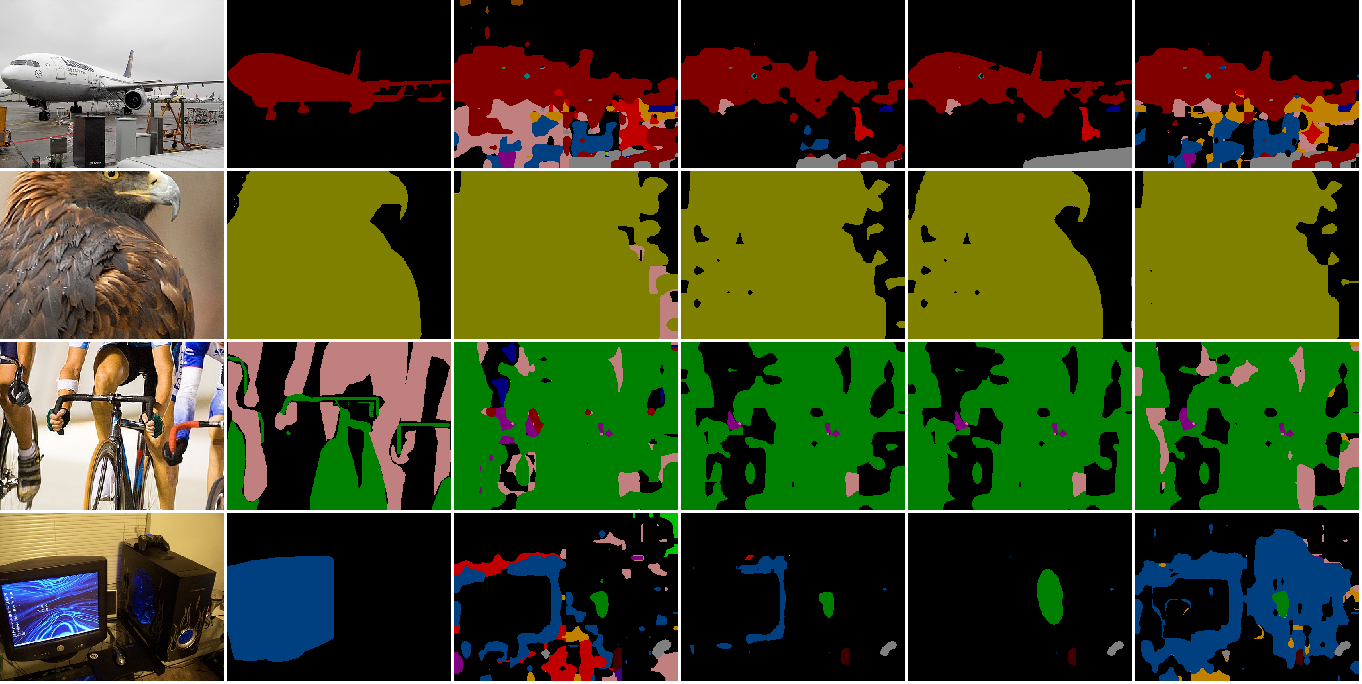
\includegraphics[width=\linewidth]{figs/reva_qual.png}
\caption{Qualitative results (NACLIP). Columns: image, GT, plain vocabulary
(pixel), plain+VABS (pixel), \reva{} (VABS+SAM), official vocabulary (pixel).
Rows 1--2: VABS suppresses plain-vocabulary false positives and SAM arbitration
cleans region boundaries. Rows 3--4 are honest failure cases: the person cyclist
is partly absorbed by negatives/bicycle, and the tvmonitor is lost by \reva{}
while the official vocabulary's engineered queries recover it---the residual
per-class harm quantified in Table~\ref{tab:perclass}.}
\label{fig:qual}
\end{figure}

\begin{figure}[t]
\centering
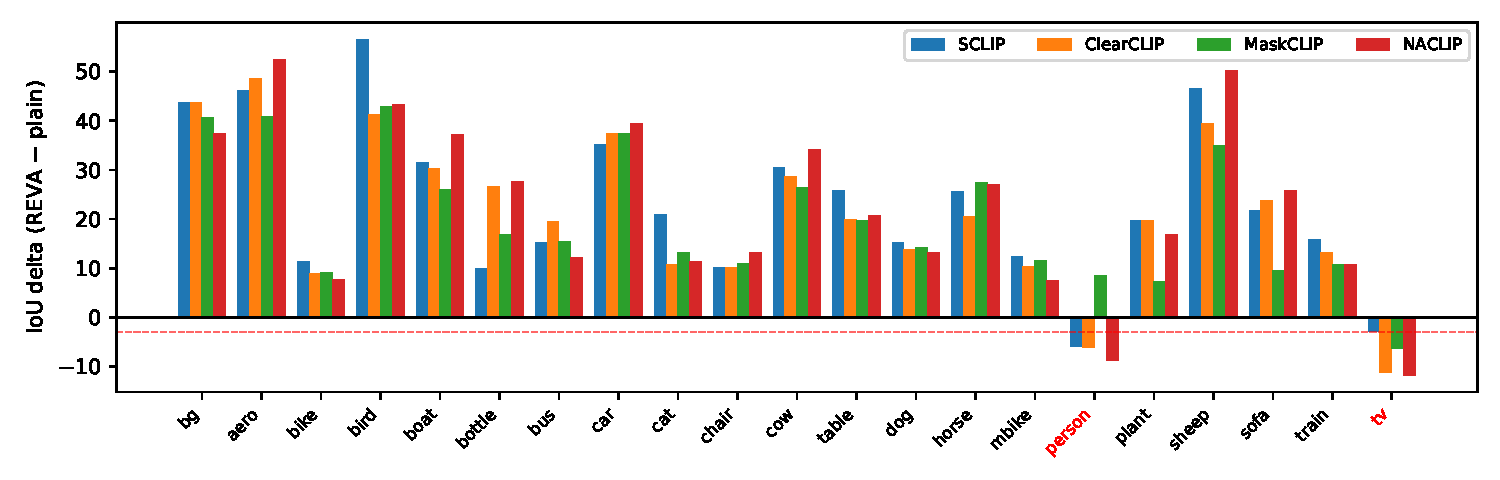
\includegraphics[width=\linewidth]{figs/reva_perclass_delta.pdf}
\caption{Per-class IoU change of \reva{} relative to the plain-vocabulary pixel
baseline (dev-excluded VOC). Every class improves on every method except
person (down on three of four methods; MaskCLIP $+8.6$) and tvmonitor (down
on all four) --- the two classes the audit identified as victims of text-only
negative synthesis (red labels); the dashed line marks $-3$ IoU.}
\label{fig:perclass}
\end{figure}

\subsection{Stage 2: visual veto (killed)}
A pre-registered second stage re-assigned background-won regions whose DINOv2 \citep{oquab2024dinov2}
embedding matched a high-confidence same-image target anchor. Best dev gain over stage
1 was $-0.08$ \miou{} (criterion: $\ge +1$); the stage is dead. Region pooling already
captures the recoverable signal; remaining background regions similar to target
anchors are predominantly true background.

\subsection{Transfer and boundary conditions}
\label{sec:transfer}
On a COCO-Object protocol (80 things + background, full val2017), the full pipeline
lifts the plain-vocabulary baseline from 22.4/22.4 to 34.4/36.3 (SCLIP/NACLIP); region
arbitration contributes $+2.5$/$+3.9$ over pixel VABS with a reduced selection
advantage ($+1.1$/$+0.8$). On PASCAL-Context-60 (full split), pooling still adds $+2.0$/$+3.1$
over pixel VABS (31.3/31.9 $\rightarrow$ 33.3/35.0; plain 31.2/31.8)
but VABS is indistinguishable from random
negatives---consistent with the audit's
finding that low-background-room regimes leave no space for negative selection.
Across benchmarks the effect tracks the size of the background-modelling room
the audit identified, as its boundary-condition model predicts: VOC-21 (26-name
engineered background expansion) $+19.9$ to $+23.1$; COCO-Object (all stuff
remapped to background) $+12.0$/$+13.9$; Context-60 (59 classes already cover
the scene) $+2.0$/$+3.1$; ADE-150 (no background channel at all) $+1.0$/$+1.3$.
\reva{} is not a one-benchmark phenomenon --- it is a repair whose available
gain is set by how much background under-modelling the target protocol has. We
retain the earlier disclosure that the scene lexicon shares names with COCO-Stuff,
which the COCO-Object protocol remaps to background: part of the negative set
coincides by construction with ground-truth background semantics on this benchmark,
so the COCO-Object transfer overstates what a fully leak-free lexicon would achieve.
Two further pre-registered transfers sharpen the boundary. On ADE-150 (150 classes,
no background class; val first-300), region arbitration still helps but shrinks to
$+1.0$/$+1.3$ over pixel VABS (SCLIP 13.13$\to$14.17, NACLIP 14.74$\to$16.06), and VABS
itself is null: no gain over plain names and indistinguishable from random
negatives---without a background class to absorb into, vocabulary-adaptive negative
selection has no room, the same mechanism as Context-60. On an OpenCLIP ViT-L/14
backbone (VOC-21 test-300), the full six-cell grid on SCLIP and NACLIP shows
the pipeline transfers: SCLIP plain 37.2 $\to$ REVA 44.0 and NACLIP plain 36.3
$\to$ REVA 51.6, in both cases \emph{above} the pixel-level official reference
(40.7 / 50.6; no matched official$+$SAM bound was run at ViT-L, and ViT-L
dense baselines are globally weaker than ViT-B). The VABS-vs-random selection
advantage is $+3.1$ on NACLIP but drops to $+1.8$ on SCLIP, below our $+2$
replication bar; VABS negatives were selected with ViT-B text embeddings and
reused unchanged.
We therefore scope the selection-advantage claim to background-rich
vocabularies, note that it is method-dependent at ViT-L scale, and observe
that region arbitration transfers in every regime tested.

Finally, REVA transfers beyond the attention-surgery family. Applied to a
ProxyCLIP-style base (DINO proxy attention over CLIP values, our
style-reimplementation of a 2024 visually-guided method; VOC-21 test-300), plain
vocabulary rises from 37.8 to 58.5 --- closing 99\% of the gap to the
pixel-level engineered-vocabulary reference (58.8), or 85\% of the gap to the
matched official$+$SAM bound (62.1), on a fifth base method whose dense
mechanism differs qualitatively from the other four --- with a $+4.2$ advantage
over matched random negatives. An external anchor on the \emph{unmodified} official ProxyCLIP release
(authors' protocol, only the class-name file swapped) confirms the text-side
component outside our stack: adding the VABS-64 negatives to the plain name
file lifts author-code \miou{} from 47.3 to 56.2, recovering 64\% of the
author-code naming-engineering gap (official name file: 61.2); the SAM
arbitration component cannot be attached without modifying their code and is
therefore not anchored. A second author-code anchor with a pre-registered
random control, the unmodified official SC-CLIP release (full VOC val):
VABS-64 lifts plain from 43.0 to 59.6 ($+16.7$, recovering 77\% of its
author-code naming-engineering gap to 64.6), while the same budget of matched
random negatives reaches 56.5 --- a $+3.1$ selection advantage on author code
(single run, single negative seed), consistent with the $+3.1$/$+3.6$
full-split means measured in our own stack (Table~\ref{tab:main}). On this
release the SAM arbitration component is anchored as well, applied as a
pre-registered \emph{additive} layer on the official probability output
(the official forward is untouched; SAM ViT-B, our frozen config; the
repo's own background threshold re-applied identically): full \reva{}
(VABS$+$SAM) reaches 63.2 from plain 43.0, recovering 93\% of the
author-code naming-engineering gap to the \emph{pixel-level} official
reference (64.6; a matched official$+$SAM bound was not run on official
code, so this percentage is not compute-matched, unlike the 85--96\%
in-stack closures), with a $+3.5$ arbitration gain (59.62$\to$63.16) over
pixel-level VABS and a $+4.2$ advantage over SAM-arbitrated matched random
negatives (58.96); plain$+$SAM alone gains only $+1.1$ (44.1), so the
arbitration gain is contingent on the recalibrated background, exactly as
in our stack. For ProxyCLIP, only the VABS component remains anchored. A
third author-code anchor tests VABS \emph{inside} a SAM-coupled pipeline:
on the unmodified official Trident release (CLIP$+$DINO splicing with
SAM-encoder aggregation and SAM refinement, full VOC val, only the
class-name file changed), VABS-64 lifts plain from 47.4 to 63.5 ($+16.0$,
recovering 82\% of its author-code naming-engineering gap to 67.1, which
reproduces the published value), with a $+2.8$ advantage over matched
random negatives (60.7) --- so the selection advantage survives even where
the host method already exploits SAM internally. This covers Trident,
previously absent from our comparisons, as a host \emph{for the VABS
component only} (pixel-level name-file folding; Trident's own SAM
refinement retained as shipped; our region arbitration was not applied on
this host). Extending the same anchor to COCO-Object (author-code
naming-engineering gap only $+3.3$): \emph{negative expansion} of either kind
reaches official parity there --- VABS 37.9 and matched random negatives 38.0
from plain 34.4 --- so the pre-registered selection-advantage criterion
\emph{fails} ($-0.0$) and the recovery cannot be credited to
vocabulary-conditioned selection. Rather than a bare failure, this is a third
independent confirmation of the gap-vs-recovery boundary (after the in-stack
dataset gradient and the below-bar LPOSS cell): where the background headroom
is small, any negative expansion suffices, and the selection advantage is a
large-headroom (VOC-like) phenomenon on author code as in our stack. A
fourth, pre-registered confirmation comes from official Trident on
COCO-Object (its author-code naming gap is only $+2.0$): there even the
VABS \emph{gain} criterion fails ($+1.3$, below our $+3$ bar) and VABS is
indistinguishable from matched random negatives (40.36 vs 40.43 from plain
39.1; selection $-0.1$) --- the boundary
prediction was stated in the preregistration before the run and held. Where
the audit finds no background headroom, \reva{} has nothing to recover;
users should consult the audit's per-dataset NEG before deploying it. The
zero-headroom end is confirmed on official Trident Context-60 (author-code
NEG only $+0.2$): there negative expansion actively \emph{harms} --- VABS
$-3.4$ and matched random $-4.1$ against plain --- reproducing on author
code the null-to-harmful ADE boundary we disclose in-stack; we make no
benefit claim from the $+0.7$ VABS-vs-random difference between two harmful
arms. A fourth official codebase, CorrCLIP \citep{zhang2025corrclip}
(ICCV~2025 oral; SAM2 region masks $+$ MetaCLIP $+$ DINO, the current
training-free performance ceiling), reproduces the recovery end of the
curve and \emph{extends} its harmful end, under the same pre-registered
thresholds (single run, single negative seed, as for the other author-code
anchors; the repository's region masks are pre-generated and identical
across arms by construction): on VOC (author-code NEG $+20.5$) VABS-64
lifts plain from 54.3 to 69.5 ($+15.2$, recovering 74\% of the gap) with a
$+3.9$ advantage over matched random negatives (65.6); on COCO-Object (NEG
only $+1.4$) both expansions actively harm (VABS $-4.1$, random $-3.3$
from plain 42.3). The frozen prediction (VABS $-$ plain below the $+3$ bar
at near-zero headroom) held, and this extends the author-code harmful
regime up to a NEG of $+1.4$ --- the largest headroom at which harm has
been observed. Note the cross-host ordering tension this exposes: CorrCLIP
harms at NEG $+1.4$ while Trident merely ties at $+2.0$, so NEG does not
monotonically order regimes \emph{across} hosts --- consistent with our
treatment of the composition heuristic as an observation, not a validated
predictor (\S\ref{sec:limitations}).
As on Trident, this covers CorrCLIP for the VABS component only.
Table~\ref{tab:dosecurve} summarises the author-code dose
curve.

\begin{table}[t]
\centering
\small
\caption{Author-code dose curve (unmodified official Trident and CorrCLIP,
full val, only the class-name file changed): the naming-engineering
headroom (NEG) determines what negative expansion can do. All values are
mIoU; selection is VABS $-$ matched random; parenthesised selection values
are differences between two harmful arms and are reported descriptively
only, with no benefit claim.}
\label{tab:dosecurve}
\begin{tabular}{lrrrr}
\toprule
Host / dataset & NEG & VABS $-$ plain & selection & regime \\
\midrule
Trident / VOC-21 & $+19.7$ & $+16.0$ & $+2.8$ & recovery $+$ selection \\
CorrCLIP / VOC-21 & $+20.5$ & $+15.2$ & $+3.9$ & recovery $+$ selection \\
Trident / COCO-Object & $+2.0$ & $+1.3$ & $-0.1$ & parity, no selection \\
CorrCLIP / COCO-Object & $+1.4$ & $-4.1$ & ($-0.8$) & harmful \\
Trident / Context-60 & $+0.2$ & $-3.4$ & ($+0.7$) & harmful \\
\bottomrule
\end{tabular}
\end{table}

The companion audit's generational extension shows
this base is exactly as naming-sensitive as the surgery family (NEG $+22.1$ on
the full dev-excluded split), so
the repair is as relevant for the newest generation as for the old.
The same protocol on two further 2024--25 style-reimplementations brings the
total to seven base methods: on SC-CLIP-style anomaly restoration, REVA lifts
plain from 38.1 to 58.5 (above its engineered-vocabulary pixel reference of
56.7, VABS-vs-random $+3.1$); on LPOSS-style label propagation it lifts plain
from 41.2 to 57.4 (94\% gap closure), but the VABS-vs-random advantage there is
only $+1.3$, below our $+2$ replication bar --- label propagation partially
absorbs the distinction between negative vocabularies, so on that family we
claim gap closure from region arbitration but not a negative-selection
advantage. Against the \emph{matched} official$+$SAM upper bounds, which we
have now run for all three bases (ProxyCLIP 62.1, LPOSS 60.3, SC-CLIP 60.9 on
the same test-300 protocol), the gap closures are 85.4\%, 85.2\% and 89.4\%
respectively; SC-CLIP REVA (58.5) exceeds its pixel-level official reference
(56.7) but remains 2.4 below the matched bound. The SC-CLIP figure of $+3.1$
is the VABS-vs-random selection advantage (58.5 vs 55.4), not the margin over
its official reference.

\subsection{Controls mandated by novelty checking}
\label{sec:controls}
Two same-protocol controls on the dev-excluded split (1349 images): (i)
\emph{LaVG-style feature pooling} (average dense features in the region, then cosine
argmax) scores 59.2/57.3/52.7/59.3 (SCLIP, ClearCLIP, MaskCLIP, NACLIP) versus our
probability pooling 58.7/56.1/52.7/59.2: feature pooling is equal or slightly better
(up to $+1.2$ on ClearCLIP), so we claim no superiority for probability pooling; its
role here is only that it operates on calibrated class probabilities, which the VABS
negatives require. (ii) \emph{Hand-written background control} (SCLIP's official
26-entry background expansion on the plain vocabulary, same SAM pooling) scores
59.0/58.4/53.0/61.0: manual engineering is equal or slightly \emph{better} (up to
$+2.3$ on ClearCLIP)---VABS's value is automation for vocabularies where no
hand-engineered expansion exists, not superior quality. A pre-registered
off-VOC check tests whether the adaptivity ever pays: transplanting the same
26-entry list verbatim to vocabularies it was not written for, VABS beats it
on COCO-Object by $+1.3$/$+2.2$ (30.48/30.65 vs 31.81/32.81 GT-present,
SCLIP/NACLIP, pixel arms, test-300), while on ADE-150 both are null-to-slightly
harmful (the disclosed ADE boundary extends to the hand list). The static list
is thus a VOC-shaped artifact; where its assumptions break, the
vocabulary-conditioned selection is what remains (single seed; both arms share
partial stuff$\to$background lexicon overlap on COCO-Object).

\paragraph{What the selection advantage is, mechanically.} A pre-registered
accounting on test-300 (region arbitration, matched random negatives) locates
the advantage: VABS raises GT-background \emph{recall} by $+5.0$/$+4.7$ points
(SCLIP 89.2 vs 84.2; NACLIP 91.2 vs 86.5) at no precision cost ($+1.3$/$+0.8$).
At pixel level, a VABS negative wins 33--36\% of pixels versus 17--19\% for
random negatives: vocabulary-conditioned negatives are competitive against
foreground classes where random words are not, so background stops leaking
into objects. The advantage is background recall, not foreground
discrimination --- consistent with the boost self-attack's finding that most
(not all) of the text-side gain is background re-calibration.

\paragraph{Perturbed-vocabulary axes.} A pre-registered check runs \reva{} on
the audit's other two axes (VOC-21 test-300, VABS negatives regenerated by the
frozen recipe conditioned on each perturbed vocabulary; baseline arm = SAM-region
pooling on the bare perturbed vocabulary). Under 100\% synonym substitution
\reva{} lifts SCLIP $32.1\to49.9$ ($+17.8$) and NACLIP $31.6\to46.8$ ($+15.2$),
retaining 85--88\% of its plain-regime gains ($+20.4$/$+17.9$): the mechanism
survives synonym perturbation, but the residual synonym cost ($\approx$7 \miou{}
below the plain-vocabulary \reva{} level) is not repaired --- \reva{} restores
background modelling, not naming quality. On an adversarially searched (ANS)
vocabulary \reva{} lifts SCLIP $15.3\to25.1$ and NACLIP $14.7\to23.9$: a real
but partial recovery, reported as a stress bound --- \reva{} is not a defense
against worst-case naming. Single seed, single substitution seed (s0). The ANS
vocabulary was searched (by the audit) on the first 100 images of the split,
which are contained in the 300-image evaluation subset used here, so the ANS
cell is an in-search-domain stress bound rather than a held-out attack.

\paragraph{External anchors.} Two reviewer-requested anchor rows on the same split:
(i) \emph{PAMR} \citep{araslanov2020}, the standard affinity-based refinement used by
published pipelines, applied to our NACLIP pixel probabilities: official vocabulary
$56.9\rightarrow62.6$ and VABS vocabulary $54.1\rightarrow58.5$, at $0.08$\,s/image.
On the official vocabulary PAMR \emph{matches} our SAM arbitration ($62.6$) at a
fraction of the cost; with VABS negatives SAM arbitration retains a $+0.7$ edge
($59.2$ vs $58.5$). We report this honestly: for engineered vocabularies cheap
affinity refinement suffices, and the specific value of region arbitration is
concentrated in the synthesized-negative regime it was designed for. It also
explains most of the reproduction gap to published NACLIP (62.6 vs 64.1; the
remainder is attributable to residual pipeline differences of the official
repository --- its resolution settings match ours, so the gap is not a
resolution artifact). (ii) \emph{Trident-style SAM refinement}
\citep{shi2025trident}: their released prompt-based refinement stage (connected
components of the coarse prediction prompt the SAM decoder with points, boxes and
mask priors) ported onto our dense probabilities with the same SAM ViT-B checkpoint;
results in Table~\ref{tab:anchor}. The two SAM-based mechanisms are close on both
vocabularies (within $0.4$ \miou{} on SCLIP in our favour, within $0.7$ against us on
NACLIP), and the prompt-based decoder pass is $\sim$3$\times$ cheaper than automask
generation. We therefore do \emph{not} claim our probability-pooling arbitration is a
superior SAM-usage mechanism; the vocabulary contribution (VABS) is orthogonal to and
composable with either. Full Trident additionally splices CLIP/DINO features and uses
SAM ViT-H at higher resolution; our row reproduces only its refinement stage under our
protocol and is an anchor, not a reproduction of their published numbers.

\begin{table}[t]
\centering\small
\begin{tabular}{llccc}
\toprule
Arbitration & Vocabulary & SCLIP & NACLIP & s/img \\
\midrule
none (pixel)            & plain+VABS & 55.5 & 54.1 & --   \\
PAMR                    & plain+VABS & --   & 58.5 & 0.09 \\
Trident SAM-refinement  & plain+VABS & 58.4 & \textbf{59.8} & 0.13 \\
\reva{} (SAM automask pooling) & plain+VABS & \textbf{58.7} & 59.2 & 0.42 \\
\midrule
none (pixel)            & official   & 57.2 & 56.9 & --   \\
PAMR                    & official   & --   & 62.6 & 0.08 \\
Trident SAM-refinement  & official   & 61.0 & \textbf{63.0} & 0.13 \\
SAM automask pooling    & official   & \textbf{61.2} & 62.6 & 0.42 \\
\bottomrule
\end{tabular}
\caption{External anchor mechanisms on the dev-excluded VOC-21 split (1349 images),
all on the same dense probabilities and (for SAM rows) the same SAM ViT-B checkpoint.
Timing is the refinement cost on top of the CLIP pass (0.035\,s). PAMR was run on
NACLIP only.}
\label{tab:anchor}
\end{table}

\subsection{A third component candidate: detector-guided vocabulary pruning}
\label{sec:prune}
This section reports a \emph{candidate} extension under evaluation; it is not
part of \reva{} proper, and no headline claim of this paper (abstract,
contributions, main tables) includes it. A pre-registered follow-up probe tests whether an external open-vocabulary
detector's \emph{box support} can prune the dense argmax: a vocabulary entry
is kept only if OWLv2 (base-ensemble, untuned threshold $0.2$) fires at
least one box for it in the image; background is always kept. Across nine
cells (\{SCLIP, ClearCLIP, NACLIP\} $\times$ \{VOC-21, Context-60,
COCO-Object\}, 300-image subsets) pruning improves the dense model by
$+1.4$ to $+9.2$ \miou{} (mean $+4.4$), harms no cell, and does not amplify
naming fragility (the synonym arm also gains; the synonym drop is unchanged,
$4.8$ vs $4.2$). It composes additively with \reva{} on all three methods
tested (VOC): SCLIP $57.0\to59.4$, ClearCLIP $54.5\to57.0$, NACLIP
$57.5\to61.1$ --- on this 300-image subset the SCLIP cell reaches $59.4$
against an engineered-vocabulary pixel reference of $58.8$ (not a
main-table claim; the main tables use the full dev-excluded split). A pixel-flow accounting suggests why the synonym arm also
gains: $55\%$ of the foreground pixels that synonym renaming leaks away
go to classes \emph{absent} from the image (only $3\%$ to present
classes), which is exactly the mass pruning removes; we report this
descriptively, as an aggregate accounting with no class-level claims ---
a class-level graded correlation between absent-leak fraction and pruning
gain did not survive pre-registered testing (Spearman $-0.20$). Two pre-registered boundary probes: on ADE-150 the
gain persists but \emph{shrinks} ($+2.5$ to $+2.7$ for SCLIP/NACLIP vs
$+6$ to $+9$ on VOC) --- it does not grow with vocabulary size as an
absent-mass account would predict --- and a pre-registered granularity
probe rules out the obvious explanation: OWLv2's per-class presence
recall does \emph{not} degrade with WordNet \citep{miller1995wordnet} label depth (Spearman
$+0.17$, wrong sign) and does not predict per-class pruning gain
($+0.05$); mean presence recall on ADE is $0.67$, i.e.\ a third of
present classes are wrongly pruned yet the net gain survives. A
bounded pixel ledger locates the shrinkage on the loss side: the
correction mass (dense-wrong pixels rescued by pruning) is nearly
constant across VOC and ADE, but the destruction mass (dense-correct
pixels whose GT class was pruned) grows $2.6$--$3.5\times$ as the
mispruned present-class share rises from $14\%$ to $34\%$ --- and the
mispruning is fault-tolerant because the detector tends to miss
exactly the classes dense CLIP already segments poorly (dense IoU
$10$--$30$ for mispruned vs $28$--$50$ for kept classes), so deletions
cost less than their count suggests; \emph{why} detector misses
concentrate there remains open (a pre-registered soft variant that
down-weights unsupported classes by $\lambda{=}0.3$ instead of deleting
them recovers $+0.6$ of the ADE loss but costs up to $1.7$ on VOC ---
a mild, not free, mitigation); a matched-budget trivial baseline ---
CLIP image-level top-$k$ filtering with $k$ set per image to the number
of classes the detector keeps --- reaches $\sim$80\% of the gain on VOC
but is \emph{net negative} on ADE-150 ($-3.9$ vs $+2.5$ to $+2.7$ for
detector pruning), so the detector evidence, not generic class
filtering, is what keeps pruning safe as the vocabulary grows; and
under the searched worst-case
vocabulary of the companion audit, pruning lifts the attacked arm by
$\sim$7 \miou{} but recovers only $\sim$35\% of the damage --- it is
not a defense against attacks that degrade the scoring of \emph{present}
classes. Honest framing: this adds a second
model at inference (an OWLv2 pass per image, a cost of the same order as
the SAM stage that already dominates our runtime), it re-imports the
detector's own vocabulary sensitivity into the pipeline (the companion
audit measures a synonym drop of 7.1 for OWLv2 --- mild, though not a
family property: Grounding DINO drops 37.6 under the same suite, so the
detector choice matters --- and \reva{}
with pruning is no longer a pure CLIP+SAM plugin), and that model is
\emph{grounding-supervised} with a
pretraining distribution that covers the benchmark classes --- pruning
imports external supervision rather than extending the training-free
recipe, consistent with the companion audit's finding that per-class
protection tracks supervision; the standalone detector pipeline remains
stronger on detection-friendly classes, so the claim is strictly
dense-vs-dense-pruned; and this is a preliminary single-seed result on
300-image subsets --- we report it as a third-component \emph{candidate},
not an established component. Notably, the same signal fails completely as
a distractor-axis shield (see the companion audit): the detector also fires
on near-distractor names; its usefulness here is pruning absent classes
from clean vocabularies, not detecting vocabulary pollution.

\subsection{A fourth component candidate: corpus-statistics negative selection with a derived budget}
\label{sec:winstat}
Like \S\ref{sec:prune}, this reports a \emph{candidate} under evaluation,
outside \reva{} proper and outside all headline claims. VABS selects
negatives by facility-location coverage of the \emph{text} embedding
space; the per-patch win-statistics diagnostic of \S\ref{sec:method}
suggests an image-side alternative: run the host once over $50$
\emph{unlabelled} images from the target domain, count how often each
candidate negative wins a background patch, and keep the most-used
negatives. Both the winner list and the budget are derived from the
statistics alone (closest prior art selects \emph{templates} for
positive classes from unlabelled-corpus entropy statistics,
FLOSS~\citep{floss2025}, or prunes \emph{foreground} vocabularies
per image~\citep{freecp2025}; concurrent TPA~\citep{tpa2026} runs the
host over a small unlabelled deployment pool and aggregates confident
patches into \emph{positive visual} prototypes --- the same
unlabelled-deployment-statistics skeleton, but on the positive/visual
side, with no negative words and no derived budget; to our knowledge
no prior work selects background \emph{negatives} from unlabelled
target-domain statistics) ---
$M^\ast$ is the smallest budget covering $90\%$ of
background wins --- replacing the free budget parameter by a single
frozen coverage constant ($90\%$, fixed before any run; a
pre-registered sweep over $80$--$95\%$ moves the result by at most
$0.8$ \miou{} on VOC and never breaks the low-headroom no-harm bound
on ADE-150). A pre-registered
evaluation (three hosts $\times$ four datasets $\times$ three disjoint
statistics windows, all disjoint from the evaluated images; matched
facility-location controls at the same $M^\ast$) passed all frozen
criteria: on VOC and COCO-Object the statistics-selected set beats the
matched text-side control by $+0.5$ to $+5.0$ \miou{} in all $18$
cells; on the low-headroom Context-60/ADE-150 boundary it never harms
beyond the frozen $0.3$ tolerance ($18/18$ cells); the derived budget is
stable across windows (within a factor $1.9$) and adapts in the right
direction, shrinking to $7$--$17$ words on ADE-150 versus $19$--$34$
elsewhere. The selected set uses roughly a third of the VABS-64 budget at
a cost of $0$--$1.1$ \miou{} (on ADE-150 it beats the full set in $6/9$
cells and is within $0.15$ in the remaining three), and the selection transfers across stacks: plugged
into the unmodified official ProxyCLIP release, statistics-selected
negatives beat the matched text-side control at the same budget by
$+1.6$ \miou{} for the derived-budget selection ($M^\ast{=}21$,
$59.2$ vs $57.7$) and $+1.5$ for the earlier fixed-$24$ registration,
both pre-registered (run records in the artifact). Caveats: single evaluation seed,
shared CLIP backbone across the three hosts, statistics windows drawn
from the same benchmark image distribution as the evaluation split
(disjoint images, same domain --- the realistic deployment assumption;
a pre-registered cross-domain probe, counting statistics on the
\emph{other} benchmark's images, still beats the matched control in all
six cells by $+1.8$ to $+4.1$ \miou{}, at $0$--$1.2$ below the
same-domain selection --- both benchmarks are natural-image
distributions, so only near-domain shift is covered and larger shifts
remain untested); an earlier registration of
this component failed one frozen gate by $0.02$ \miou{} and is reported
in the artifact alongside this re-registration; the re-registration
dropped that gate's plain-relative condition (a post-hoc verification
finds it would have passed in all $36$ cells here) and pre-committed a
one-miss-per-dataset tolerance that the results did not need. A final
pre-registered promotion gate (official ProxyCLIP, Context-60, plain
vocabulary) \emph{failed}: while the statistics selection again matches
the text-side control ($33.7$ vs $34.0$, within the $0.3$ tolerance),
\emph{any} negative expansion harms this low-headroom cell relative to
plain ($36.5$) by ${\sim}2.8$ \miou{} --- consistent with the
applicability boundary of \S\ref{sec:transfer}, and the reason this
component remains a candidate outside \reva{} proper: it improves
\emph{which} negatives to use, not \emph{whether} to use them.

\section{Limitations}
\label{sec:limitations}
Same-protocol anchors now cover Trident's SAM-refinement stage and PAMR
(Table~\ref{tab:anchor}); they show our arbitration is competitive but not uniformly
superior, and a TCC comparison and full-Trident reproduction (CLIP/DINO splicing, SAM
ViT-H, higher resolution) remain unrun, so our absolute numbers are still not
comparable to published multi-scale pipelines (see \S\ref{sec:prereg}). Single backbone
(ViT-B/16); SAM adds an external visual model whose automatic mask generation
dominates runtime: measured per-image cost is $0.42$\,s for SAM + pooling versus
$0.035$\,s for the CLIP dense pass ($\sim$12$\times$; RTX 3090, points-per-side 16).
The matched random-negative control is now replicated with 3 seeds at
full-split scale (all cells positive; Table~\ref{tab:main}); other controls
remain single-seed as noted. The author-code anchors validate VABS on four
official releases (ProxyCLIP, SC-CLIP, Trident, CorrCLIP) and full \reva{}
(VABS$+$SAM, additive on the official probability output) on one (SC-CLIP,
VOC); the arbitration layer has not been run as a \emph{replacement} for
any official repository's own postprocess, and the ProxyCLIP anchor covers
VABS only. A pre-registered \emph{additive} redundancy test on one further
official release bounds where arbitration helps: applied on top of
official CorrCLIP --- whose shipped postprocess already mode-votes over
its pre-generated SAM2 regions --- our layer fails the pre-registered
$\geq+1.0$ transfer criterion (VOC, single run: VABS arm $69.5 \to 68.2$,
$-1.3$ vs the official postprocess; matched random arm $65.6 \to 64.1$,
$-1.6$; both small negative deltas are reported descriptively, no harm
claim), matching the pre-registered frozen prediction of
failure/redundancy. This is consistent with arbitration adding value only
where the host has not already aggregated region evidence --- a
single-dataset boundary observation on one host pair, not a validated
host-level rule. OpenReview-stage collision checking was
unavailable (provisional novelty). \textbf{Applicability warning}: the
author-code dose curve (Trident VOC NEG $+19.7 \to$ VABS $+16.0$;
Trident COCO-Object $+2.0 \to$ tie; CorrCLIP COCO-Object $+1.4 \to$ VABS
\emph{harms}, $-4.1$; Trident Context-60 $+0.2 \to$ VABS \emph{harms},
$-3.4$) means
\reva{} should not be deployed on low-headroom regimes --- benchmarks whose
vocabulary already densely covers scene content (stuff-inclusive label
spaces where background is a minor residual class), as opposed to
thing-centric vocabularies with a large residual background. This
composition heuristic is consistent with every measured point but is a
post-hoc observation, not a validated predictor; an automatic, deploy-time
applicability test (the user cannot measure NEG without an engineered
vocabulary) is an open problem. A pre-registered pilot on this problem
found one label-free signal with the pre-declared sign: vocabulary
\emph{crowding} (mean max image--query cosine similarity on 50 unlabelled
images) anti-correlates with the oracle expansion gain across 8
host--dataset configurations (Spearman $-0.69$ with primary-source
gains; the two hosts share four datasets, so the effective sample is
closer to 4 and the pass over the frozen $0.6$ bar is thin); prediction
entropy,
despite correlating more strongly, has the \emph{wrong} pre-declared sign
(confounded by vocabulary size) and a frozen global-threshold switch
failed its do-no-harm criterion (host-dependent signal scales), so we
report a candidate signal, not a validated detector. A pre-registered
ordinal out-of-sample check on the official codebases (read-only crowding
margin from each repo's stored class map, 50 unlabelled images, single
run) ordered 4 of 5 within-host dataset pairs correctly ($n=5$ pairs),
with the single miss coming from the repo with the deepest stored
post-processing; by the frozen criterion this is marginal and carries no
claim. A pre-registered expansion under a single matched extraction
protocol (raw cosine, 18 points: three hosts $\times$ four datasets
plus synonym-substituted vocabularies on two of them) passed both its
pooled and per-host bars (pooled Spearman $-0.72$; $-0.83$ within
every host --- the host-scale confound that broke the global switch
does not break the within-host ordering; the three hosts share the
CLIP backbone and produce \emph{identical} rank orderings, so this is
one within-host test replicated three times, not three independent
replications), but its vocabulary-axis
test failed $0/6$: within a fixed dataset, replacing class names by
synonyms lowers both the crowding score and the expansion gain, the
\emph{opposite} of the frozen prediction. The signal is therefore a
dataset-level headroom proxy that must be calibrated per host, not a
vocabulary-level one; for synonym substitution it cannot see
naming-induced headroom changes --- a pre-registered robustness check
over two additional random second-tier synonym draws replicated the
inverted pattern in all $12$ of $12$ plain-vs-synonym pairs (three
hosts $\times$ two datasets $\times$ two draws). A
pre-registered ViT-L/14 replication did not clear its frozen bar
(one host $-0.89$, the other $-0.49$ against a $-0.5$ bar, and the
crowding ordering coincides with ViT-B/16's, so backbone independence
remains unestablished); the signal stays a pilot. Development images come from VOC; cross-dataset hyper-parameter
transfer beyond the reported protocols is untested. Finally, a pre-registered
attempt to \emph{amortise} \reva{} into a learned text-side adapter with universal
background queries (trained on 8k unlabelled ADE images with \reva{} pseudo-labels
and a naming-invariance loss) failed all its criteria: universal learned negatives
cannot contain vocabulary-relative words (sky/grass are VOC negatives but training
targets), and invariance training degraded held-out synonym vocabularies. The
vocabulary-adaptivity of VABS at inference time appears essential, and \reva{}'s
inference cost cannot currently be trained away on the text side (records in the
companion audit's artifact). A follow-up probe that moved the same
naming-invariance objective to a visual-side adapter over frozen dense features
also failed its pre-registered criteria (held-out synonym vocabularies degraded,
the same failure signature), and a per-region configuration-routing oracle showed
a $+14.9$ \miou{} ceiling that no label-free gate we tested could access; both are
reported in the companion audit as negative results; a follow-up router fit on 50
labelled images also failed to beat the best fixed configuration, so the routing
ceiling remains inaccessible to every signal family we tested. ADE-150 and ViT-L/14
transfers (\S\ref{sec:transfer}) bound the applicability of negative selection to
background-rich vocabularies, with a method-dependent advantage at ViT-L scale.

\section{Conclusion}
\reva{} turns the audit's negative result into a largely constructive one: region
evidence arbitration prevents the \emph{additional} per-class harm that killed
text-only negative synthesis, and recovers 86--96\% of the engineered-vocabulary gap
under matched compute, under pre-registered criteria and matched controls. What it
does not do is also reported: the residual harm to person and tvmonitor relative to
the plain baseline is reduced but not eliminated, the engineered vocabulary retains a
0.9--3.6 \miou{} lead at matched compute, and SAM dominates inference cost. The
per-class protective component of engineered vocabularies thus remains only
partially automatable---a refined version of the audit's open problem.

\appendix
\section{Per-class IoU on the dev-excluded VOC split}
\label{app:perclass}

Table~\ref{tab:perclass} reports the full per-class breakdown behind the
safety criterion of \S\ref{sec:prereg}.

\begin{table}[h]
\centering\scriptsize
\caption{Per-class IoU (\%) on the dev-excluded VOC-21 split: plain-vocabulary pixel
baseline (pl), pixel-level VABS (pix), and \reva{} (+SAM). The pre-registered safety
criterion compares +SAM against pix (arbitration adds no harm; worst single-method
regression person $-3.2$ on NACLIP). Against pl, the harm inherited from text-only
negative synthesis persists for tvmonitor on all four methods and for person
on three of four (MaskCLIP $+8.6$; bounded at $-11.8$).}
\label{tab:perclass}
\begin{tabular}{lcccccccccccc}
\toprule
& \multicolumn{3}{c}{SCLIP} & \multicolumn{3}{c}{ClearCLIP} & \multicolumn{3}{c}{MaskCLIP} & \multicolumn{3}{c}{NACLIP} \\
\cmidrule(lr){2-4}\cmidrule(lr){5-7}\cmidrule(lr){8-10}\cmidrule(lr){11-13}
Class & pl & pix & +SAM & pl & pix & +SAM & pl & pix & +SAM & pl & pix & +SAM \\
\midrule
background & 40.9 & 83.0 & 84.7 & 38.9 & 80.8 & 82.5 & 43.4 & 80.0 & 84.1 & 48.3 & 83.6 & 85.7 \\
aeroplane & 14.6 & 52.3 & 60.8 & 17.6 & 53.8 & 66.1 & 12.3 & 33.2 & 53.3 & 23.6 & 59.4 & 76.0 \\
bicycle & 17.5 & 28.9 & 29.0 & 21.5 & 30.5 & 30.4 & 20.8 & 28.3 & 30.0 & 26.1 & 33.5 & 33.7 \\
bird & 21.7 & 70.9 & 78.3 & 39.0 & 71.5 & 80.3 & 22.3 & 52.0 & 65.1 & 37.1 & 70.1 & 80.3 \\
boat & 7.9 & 34.6 & 39.5 & 8.9 & 34.5 & 39.3 & 6.2 & 21.4 & 32.3 & 9.4 & 39.0 & 46.5 \\
bottle & 55.2 & 57.0 & 65.1 & 42.3 & 59.0 & 68.9 & 33.7 & 37.4 & 50.6 & 38.9 & 55.9 & 66.6 \\
bus & 70.9 & 80.3 & 86.1 & 61.6 & 73.4 & 81.2 & 56.6 & 57.4 & 72.1 & 66.4 & 68.2 & 78.5 \\
car & 35.1 & 68.1 & 70.3 & 28.2 & 63.1 & 65.6 & 25.9 & 52.0 & 63.3 & 31.3 & 65.6 & 70.7 \\
cat & 64.5 & 82.2 & 85.4 & 62.3 & 74.7 & 73.1 & 68.7 & 74.1 & 81.9 & 73.3 & 81.2 & 84.8 \\
chair & 19.2 & 27.1 & 29.4 & 18.6 & 27.3 & 28.7 & 22.4 & 26.7 & 33.4 & 17.3 & 26.3 & 30.6 \\
cow & 46.6 & 73.7 & 77.2 & 41.9 & 67.1 & 70.6 & 46.8 & 61.8 & 73.3 & 42.7 & 69.2 & 76.8 \\
diningtable & 16.9 & 41.4 & 42.6 & 20.9 & 39.0 & 40.8 & 12.8 & 27.8 & 32.5 & 20.0 & 38.5 & 40.7 \\
dog & 67.7 & 79.4 & 82.9 & 62.5 & 74.5 & 76.4 & 60.5 & 67.0 & 74.8 & 67.7 & 76.1 & 80.9 \\
horse & 36.1 & 59.2 & 61.8 & 33.7 & 52.1 & 54.1 & 34.7 & 54.3 & 62.0 & 38.9 & 61.4 & 65.9 \\
motorbike & 51.8 & 61.9 & 64.3 & 55.6 & 61.7 & 65.9 & 42.3 & 47.2 & 53.9 & 56.3 & 58.7 & 63.7 \\
person & 44.2 & 39.0 & 38.2 & 52.3 & 48.2 & 46.3 & 24.7 & 34.2 & 33.3 & 48.2 & 42.5 & 39.3 \\
pottedplant & 17.6 & 35.8 & 37.4 & 9.9 & 28.2 & 29.6 & 21.4 & 28.1 & 28.7 & 9.5 & 25.4 & 26.4 \\
sheep & 23.5 & 66.9 & 70.1 & 16.8 & 51.8 & 56.2 & 38.5 & 63.6 & 73.5 & 18.2 & 61.3 & 68.4 \\
sofa & 25.8 & 43.3 & 47.5 & 23.9 & 44.4 & 47.6 & 34.8 & 37.2 & 44.4 & 27.2 & 47.5 & 53.0 \\
train & 39.8 & 54.6 & 55.6 & 40.8 & 52.3 & 53.9 & 37.0 & 44.1 & 47.7 & 46.2 & 54.6 & 57.0 \\
tvmonitor & 29.8 & 25.7 & 26.9 & 32.4 & 23.2 & 21.2 & 22.3 & 18.4 & 16.0 & 29.2 & 18.6 & 17.4 \\
\bottomrule
\end{tabular}
\end{table}

\section{Run provenance}
All numbers derive from JSON run records stored with the code
(\texttt{runs/clean\_*.json} for the dev-excluded VOC split,
\texttt{runs/full\_*.json} for the transfer protocols); every table cell is traceable
to a specific record. Timing is recorded per run. The 100 development images
(validation indices 300--399) are excluded from every VOC test number in this paper;
earlier pre-registered dev decisions used only those images.

\bibliographystyle{plainnat}
\begin{thebibliography}{99}

\bibitem[Zhou et al.(2022)]{zhou2022maskclip}
C.~Zhou, C.~C. Loy, B.~Dai.
\newblock Extract free dense labels from CLIP.
\newblock In \emph{ECCV}, 2022.

\bibitem[Wang et al.(2024)]{wang2024sclip}
F.~Wang, J.~Mei, A.~Yuille.
\newblock SCLIP: Rethinking self-attention for dense vision-language inference.
\newblock In \emph{ECCV}, 2024.

\bibitem[Lan et al.(2024{\natexlab{a}})]{lan2024clearclip}
M.~Lan, C.~Chen, Y.~Ke, X.~Wang, L.~Feng, W.~Zhang.
\newblock ClearCLIP: Decomposing CLIP representations for dense vision-language
  inference.
\newblock In \emph{ECCV}, 2024.

\bibitem[Hajimiri et al.(2024)]{hajimiri2024naclip}
S.~Hajimiri, I.~Ben~Ayed, J.~Dolz.
\newblock Pay attention to your neighbours: Training-free open-vocabulary semantic
  segmentation.
\newblock In \emph{WACV}, 2025.

\bibitem[Lan et al.(2024{\natexlab{b}})]{lan2024proxyclip}
M.~Lan, C.~Chen, Y.~Ke, X.~Wang, L.~Feng, W.~Zhang.
\newblock ProxyCLIP: Proxy attention improves CLIP for open-vocabulary segmentation.
\newblock In \emph{ECCV}, 2024.

\bibitem[Araslanov and Roth(2020)]{araslanov2020}
N.~Araslanov, S.~Roth.
\newblock Single-stage semantic segmentation from image labels.
\newblock In \emph{CVPR}, 2020.

\bibitem[Radford et al.(2021)]{radford2021clip}
A.~Radford et al.
\newblock Learning transferable visual models from natural language supervision.
\newblock In \emph{ICML}, 2021.

\bibitem[Kirillov et al.(2023)]{kirillov2023sam}
A.~Kirillov et al.
\newblock Segment anything.
\newblock In \emph{ICCV}, 2023.

\bibitem[Sam(2026)]{sam2026fragile}
T.~Sam.
\newblock How fragile is your vocabulary? A controlled audit of inference-vocabulary
  robustness in training-free open-vocabulary semantic segmentation.
\newblock Preprint, 2026.

\bibitem[Sun et al.(2024)]{sun2024car}
S.~Sun, R.~Li, P.~Torr, X.~Gu, S.~Li.
\newblock CLIP as RNN: Segment countless visual concepts without training endeavor.
\newblock In \emph{CVPR}, 2024.

\bibitem[Karazija et al.(2024)]{karazija2024ovdiff}
L.~Karazija, I.~Laina, A.~Vedaldi, C.~Rupprecht.
\newblock Diffusion models for open-vocabulary segmentation.
\newblock In \emph{ECCV}, 2024.

\bibitem[Kang and Cho(2024)]{kang2024lavg}
D.~Kang, M.~Cho.
\newblock In defense of lazy visual grounding for open-vocabulary semantic
  segmentation.
\newblock In \emph{ECCV}, 2024.

\bibitem[Shi et al.(2025)]{shi2025trident}
Y.~Shi, M.~Dong, C.~Xu.
\newblock Harnessing vision foundation models for high-performance, training-free
  open vocabulary segmentation.
\newblock In \emph{ICCV}, 2025.

\bibitem[Zhang et al.(2025)]{zhang2025corrclip}
D.~Zhang, F.~Liu, Q.~Tang.
\newblock {CorrCLIP}: Reconstructing patch correlations in {CLIP} for
  open-vocabulary semantic segmentation.
\newblock In \emph{ICCV}, 2025.

\bibitem[Wang et al.(2024)]{wang2024samclip}
H.~Wang et al.
\newblock SAM-CLIP: Merging vision foundation models towards semantic and spatial
  understanding.
\newblock In \emph{CVPRW}, 2024.

\bibitem[Yuan et al.(2024)]{yuan2024ovsam}
H.~Yuan et al.
\newblock Open-vocabulary SAM: Segment and recognize twenty-thousand classes
  interactively.
\newblock In \emph{ECCV}, 2024.

\bibitem[Lee et al.(2025)]{lee2025escnet}
S.~Lee et al.
\newblock Effective SAM combination for open-vocabulary semantic segmentation.
\newblock In \emph{CVPR}, 2025.

\bibitem[Wysocza\'nska et al.(2025)]{tcc2024}
M.~Wysocza\'nska, A.~Vobecky, A.~Cardiel, T.~Trzci\'nski, R.~Marlet,
A.~Bursuc, O.~Sim\'eoni.
\newblock Test-time contrastive concepts for open-world semantic segmentation.
\newblock \emph{TMLR}, 2025 (arXiv:2407.05061).

\bibitem[Stojni\'c et al.(2025)]{stojnic2025lposs}
V.~Stojni\'c, Y.~Kalantidis, G.~Tolias.
\newblock LPOSS: Label propagation over patches and pixels for open-vocabulary
  semantic segmentation.
\newblock In \emph{CVPR}, 2025.

\bibitem[Chen et~al.(2025)]{freecp2025}
Q.~Chen, L.~Yang, Y.~Chen, N.~Zhao, J.~Lai, J.~Shao, X.~Xie.
\newblock FreeCP: Training-free class purification for open-vocabulary
  semantic segmentation.
\newblock In \emph{ICCV}, 2025.

\bibitem[Benigmim et~al.(2025)]{floss2025}
Y.~Benigmim, M.~Fahes, T.-H. Vu, A.~Bursuc, R.~de~Charette.
\newblock FLOSS: Free lunch in open-vocabulary semantic segmentation.
\newblock In \emph{ICCV}, 2025 (arXiv:2504.10487).

\bibitem[Tran and Shen(2026)]{activesam2026}
D.~T. Tran, Z.~Shen.
\newblock ActiveSAM: Image-conditional class pruning for fast and accurate
  open-vocabulary segmentation.
\newblock arXiv:2606.16996, 2026.

\bibitem[Wang et~al.(2026)]{tpa2026}
H.~Wang, J.~Cheng, W.~Li, X.~Tang.
\newblock Test-time prototype adaptation for open-vocabulary semantic
  segmentation.
\newblock arXiv:2608.08290, 2026.

\bibitem[Ma et~al.(2026)]{ptc2026}
W.~Ma, J.~Lu, Q.~Peng, X.~You.
\newblock Perceptual anchoring: Prototype-guided text calibration for
  training-free open-vocabulary semantic segmentation.
\newblock arXiv:2608.03991, 2026.

\bibitem[Xie et~al.(2026)]{wang2026synclip}
M.~Xie, G.~He, D.~Xu, Y.~Lin, H.~Li, P.~Feng, J.~Guan.
\newblock SynCLIP: Synonym-coherent language-image pretraining for robust
  open-vocabulary dense perception.
\newblock arXiv:2607.11008, 2026.

\bibitem[Bai et al.(2024)]{bai2024scclip}
S.~Bai, Y.~Liu, Y.~Han, H.~Zhang, Y.~Tang.
\newblock Self-calibrated CLIP for training-free open-vocabulary
  segmentation.
\newblock arXiv:2411.15869, 2024.

\bibitem[Everingham et al.(2010)]{everingham2010voc}
M.~Everingham, L.~Van~Gool, C.~K.~I. Williams, J.~Winn, and A.~Zisserman.
\newblock The {PASCAL} visual object classes ({VOC}) challenge.
\newblock \emph{IJCV}, 88(2):303--338, 2010.

\bibitem[Mottaghi et al.(2014)]{mottaghi2014context}
R.~Mottaghi, X.~Chen, X.~Liu, N.-G. Cho, S.-W. Lee, S.~Fidler, R.~Urtasun, and
  A.~Yuille.
\newblock The role of context for object detection and semantic segmentation
  in the wild.
\newblock In \emph{CVPR}, 2014.

\bibitem[Lin et al.(2014)]{lin2014coco}
T.-Y. Lin, M.~Maire, S.~Belongie, J.~Hays, P.~Perona, D.~Ramanan,
  P.~Doll\'ar, and C.~L. Zitnick.
\newblock Microsoft {COCO}: Common objects in context.
\newblock In \emph{ECCV}, 2014.

\bibitem[Caesar et al.(2018)]{caesar2018cocostuff}
H.~Caesar, J.~Uijlings, and V.~Ferrari.
\newblock {COCO-Stuff}: Thing and stuff classes in context.
\newblock In \emph{CVPR}, 2018.

\bibitem[Zhou et al.(2017)]{zhou2017ade}
B.~Zhou, H.~Zhao, X.~Puig, S.~Fidler, A.~Barriuso, and A.~Torralba.
\newblock Scene parsing through {ADE20K} dataset.
\newblock In \emph{CVPR}, 2017.

\bibitem[Ilharco et al.(2021)]{ilharco2021openclip}
G.~Ilharco, M.~Wortsman, R.~Wightman, C.~Gordon, N.~Carlini, R.~Taori,
  A.~Dave, V.~Shankar, H.~Namkoong, J.~Miller, H.~Hajishirzi, A.~Farhadi, and
  L.~Schmidt.
\newblock {OpenCLIP}.
\newblock Zenodo, 2021. \url{https://doi.org/10.5281/zenodo.5143773}.

\bibitem[Miller(1995)]{miller1995wordnet}
G.~A. Miller.
\newblock {WordNet}: A lexical database for {English}.
\newblock \emph{Communications of the ACM}, 38(11):39--41, 1995.

\bibitem[Oquab et al.(2024)]{oquab2024dinov2}
M.~Oquab, T.~Darcet, T.~Moutakanni, H.~Vo, M.~Szafraniec, V.~Khalidov,
  P.~Fernandez, D.~Haziza, F.~Massa, A.~El-Nouby, et~al.
\newblock {DINOv2}: Learning robust visual features without supervision.
\newblock \emph{TMLR}, 2024.

\bibitem[Krause and Golovin(2014)]{krause2014submodular}
A.~Krause and D.~Golovin.
\newblock Submodular function maximization.
\newblock In \emph{Tractability: Practical Approaches to Hard Problems}.
  Cambridge University Press, 2014.

\bibitem[Zhou et al.(2022{\natexlab{b}})]{zhou2022coop}
K.~Zhou, J.~Yang, C.~C. Loy, and Z.~Liu.
\newblock Learning to prompt for vision-language models.
\newblock \emph{IJCV}, 130(9):2337--2348, 2022.

\bibitem[Pratt et al.(2023)]{pratt2023cupl}
S.~Pratt, I.~Covert, R.~Liu, and A.~Farhadi.
\newblock What does a platypus look like? {G}enerating customized prompts for
  zero-shot image classification.
\newblock In \emph{ICCV}, 2023.

\bibitem[Roth et al.(2023)]{roth2023waffle}
K.~Roth, J.~M. Kim, A.~S. Koepke, O.~Vinyals, C.~Schmid, and Z.~Akata.
\newblock Waffling around for performance: Visual classification with random
  words and broad concepts.
\newblock In \emph{ICCV}, 2023.

\bibitem[Li et al.(2022)]{li2022lseg}
B.~Li, K.~Q. Weinberger, S.~Belongie, V.~Koltun, and R.~Ranftl.
\newblock Language-driven semantic segmentation.
\newblock In \emph{ICLR}, 2022.

\bibitem[Xu et al.(2022)]{xu2022groupvit}
J.~Xu, S.~De~Mello, S.~Liu, W.~Byeon, T.~Breuel, J.~Kautz, and X.~Wang.
\newblock {GroupViT}: Semantic segmentation emerges from text supervision.
\newblock In \emph{CVPR}, 2022.

\bibitem[Liang et al.(2023)]{liang2023ovseg}
F.~Liang, B.~Wu, X.~Dai, K.~Li, Y.~Zhao, H.~Zhang, P.~Zhang, P.~Vajda, and
  D.~Marculescu.
\newblock Open-vocabulary semantic segmentation with mask-adapted {CLIP}.
\newblock In \emph{CVPR}, 2023.

\bibitem[Xu et al.(2023)]{xu2023san}
M.~Xu, Z.~Zhang, F.~Wei, H.~Hu, and X.~Bai.
\newblock Side adapter network for open-vocabulary semantic segmentation.
\newblock In \emph{CVPR}, 2023.

\bibitem[Cho et al.(2024)]{cho2024catseg}
S.~Cho, H.~Shin, S.~Hong, A.~Arnab, P.~H. Seo, and S.~Kim.
\newblock {CAT-Seg}: Cost aggregation for open-vocabulary semantic
  segmentation.
\newblock In \emph{CVPR}, 2024.

\end{thebibliography}

\end{document}
